\documentclass[12pt,letterpaper,titlepage]{article}
\usepackage{fontspec}
\defaultfontfeatures{Mapping=tex-text}
\usepackage{xunicode}
\usepackage{xltxtra}
\usepackage{amsmath}
\usepackage{pdfpages}
\usepackage{amsfonts}
\usepackage{amssymb}
\setcounter{secnumdepth}{0}
\usepackage{nameref}

\setmainfont{Times New Roman}
\showboxdepth=\maxdimen
\showboxbreadth=\maxdimen

\usepackage[tocflat]{tocstyle}
\usetocstyle{allwithdot}
\usepackage[bottom]{footmisc}

\usepackage{karnaugh-map}
\usepackage{paracol}
\usepackage{wrapfig}
\globalcounter{table}
\globalcounter{figure}
\usepackage{graphicx}
\usepackage[left=1in,right=1in,top=1in,bottom=1in]{geometry}
\graphicspath{{img/}}
\author{Jacob Abel}
\title{Project 3}

\setlength{\parskip}{0.5em}


\begin{document}
\maketitle


\tableofcontents
\pagebreak
\listoftables

\listoffigures

\pagebreak
\begin{raggedright}

\section{Purpose}


\section{Problem Specification}


\section{Disassembly and Initial Analysis}

\begin{table}[ht]
\centering
\begin{tabular}{|c|c|l|} \hline 
Memory Address & Machine Code & Instruction (Values in decimal) \\ \hline 
0 & 1400 & XOR R0, R0, R0   \\ \hline 
1 & 2100 & LD  R4, R0       \\ \hline 
2 & 8443 & ADI R1, R0, 3   \\ \hline 
3 & 0480 & ADD R2, R0, R0   \\ \hline 
4 & 00E0 & MOV R3, R4       \\ \hline 
5 & 0290 & INC R2, R2       \\ \hline 
6 & 0ADA & SUB R3, R3, R2   \\ \hline 
7 & 0C48 & DEC R1, R1       \\ \hline 
8 & C00A & BRZ R0, R1       \\ \hline 
9 & C1C4 & BRZ R7, R0       \\ \hline 
A & 02D8 & INC R3, R3       \\ \hline 
B & 0C48 & DEC R1, R1       \\ \hline 
C & 1A41 & SHR R1, R1       \\ \hline 
D & C20A & BRN R0, R1       \\ \hline 
E & E000 & JMP R0           \\ \hline 
\end{tabular} 
\caption{Step 1: Initial Instruction Disassembly}\label{step1}
\end{table}

\section{Design Process}


\section{Implementation}


\section{Validation}


\section{Conclusion}


\clearpage

\section{Appendix A: Simulation Waveforms}

\clearpage

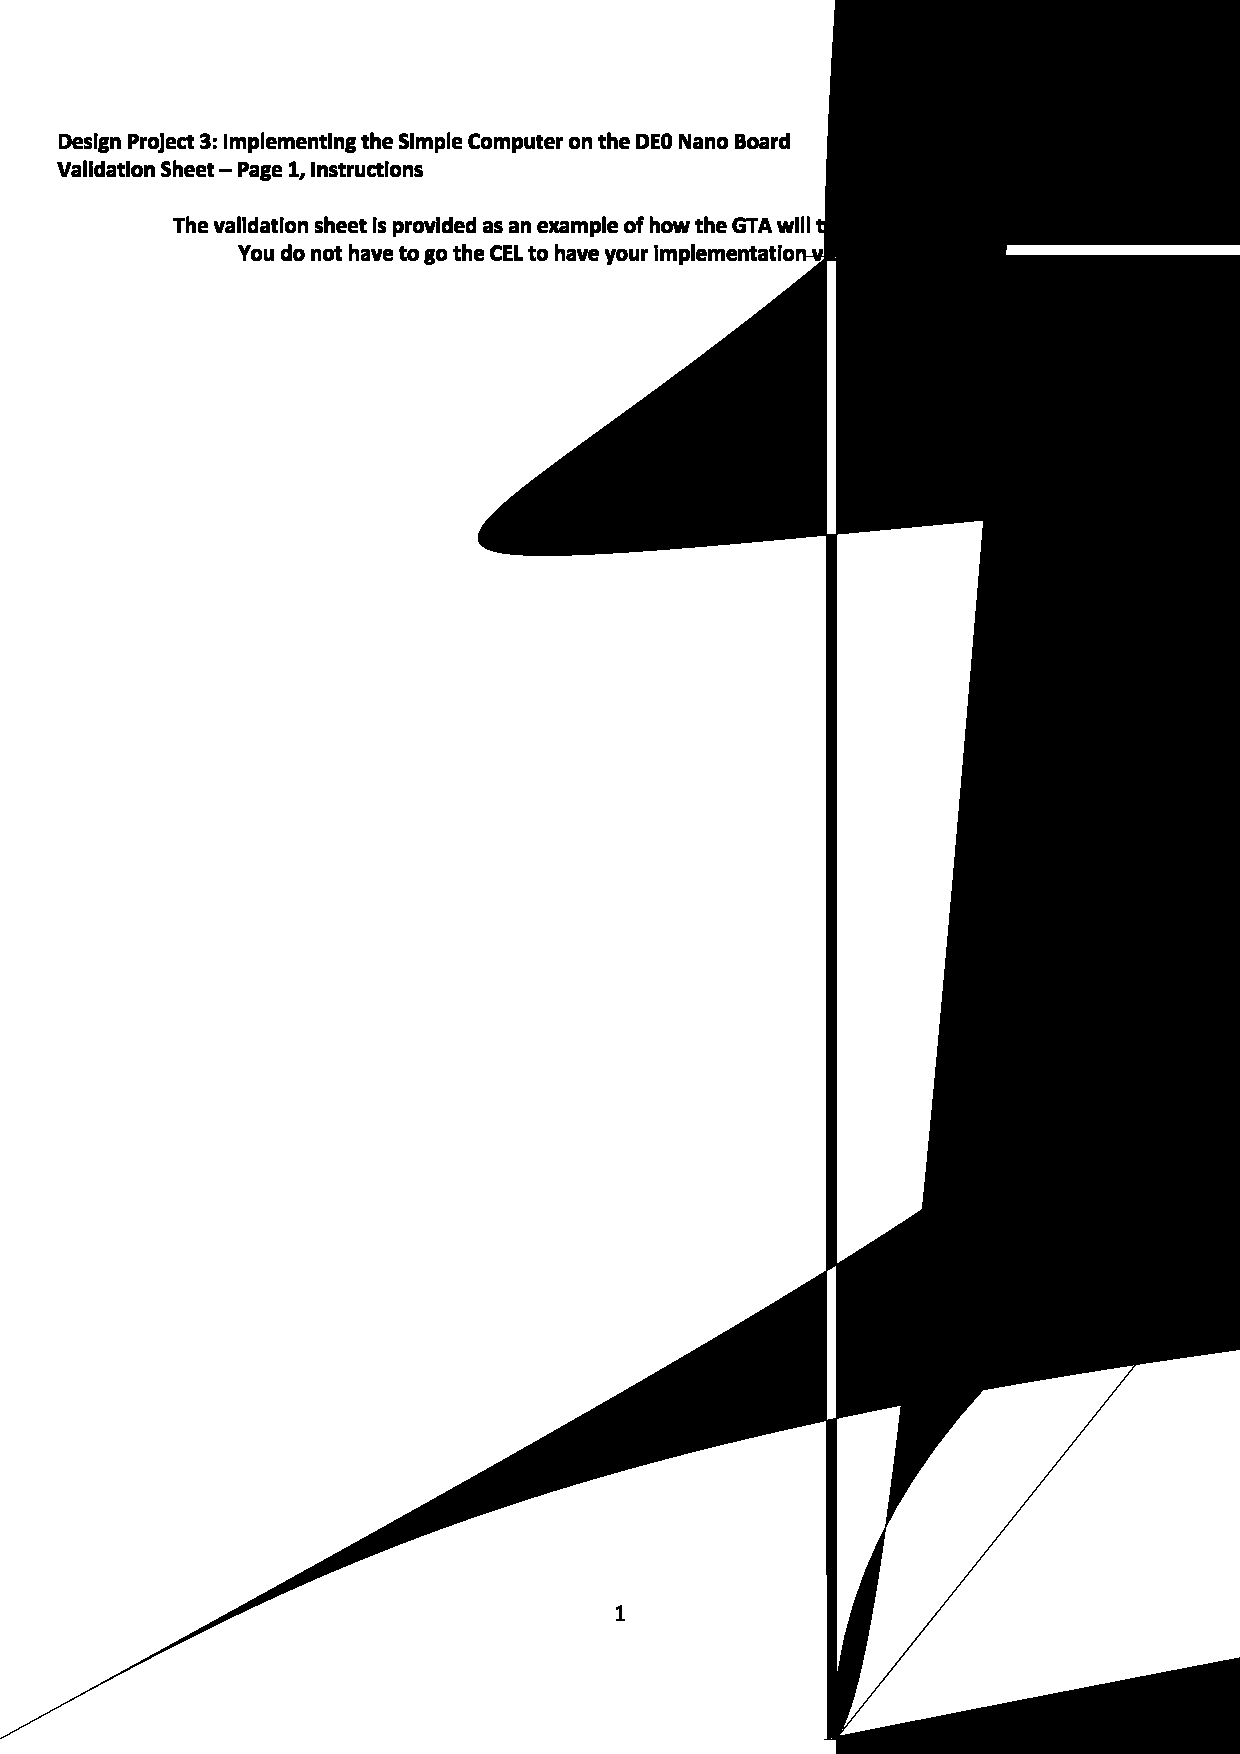
\includepdf[pages=-, noautoscale]{ValSheet.pdf}

\end{raggedright}
\end{document}
